%% bourque_cosc880.tex
%% Matthew Bourque

\documentclass[10pt,journal,compsoc]{IEEEtran}

% imports
\usepackage{graphicx}
\usepackage{hyperref}
\usepackage{listings}

% *** CITATION RELATED PACKAGES ***
\ifCLASSOPTIONcompsoc
  \usepackage[nocompress]{cite}
\else
  \usepackage{cite}
\fi

% correct bad hyphenation here
\hyphenation{op-tical net-works semi-conduc-tor}


\begin{document}

% Title
\title{The Hubble Space Telescope (HST) Advanced Camera for Surveys (ACS) Quicklook Project}

% Authors
\author{Matthew~Bourque[1], Sara~Ogaz[1], Alex~Viana[2], Meredith~Durbin[3], Norman Grogin[1]\\
\begin{flushleft}
{\scriptsize [1] Space Telescope Science Institute, Baltimore, Maryland 21218. email: bourque@stsci.edu, ogaz@stsci.edu, grogin@stsci.edu}\\
{\scriptsize [2] Dept. of Astronomy, The University of Washington, Box 351580, U.W. Seattle, Washington, 98195, email:mdurbin@uw.edu}\\
{\scriptsize [3] Terbium Labs, Baltimore, Maryland 21201. email: alexcostaviana@gmail.com}
\end{flushleft}
\IEEEcompsocitemizethanks{\IEEEcompsocthanksitem M. Bourque, S. Ogaz, A. Viana, and
M. Durbin were with the Space Telescope Science Institute, Baltimore, MD, 21218.
\protect\\
E-mail: bourque@stsci.edu}
\thanks{Manuscript received Month DD, YYYY}}

% Abstract
\IEEEtitleabstractindextext{%
\begin{abstract}
What is an abstract, really?
\end{abstract}}


% make the title area
\maketitle
\IEEEdisplaynontitleabstractindextext
\IEEEpeerreviewmaketitle


% Introduction
\IEEEraisesectionheading{\section{Introduction}\label{sec:introduction}}
\IEEEPARstart The Advanced Camera for Surveys (ACS) is a third-generation imaging
instrument on board the Hubble Space Telescope (HST), installed in 2002 during
Servicing Mission 3B. It is comprised of three detectors: (1) the Wide Field Camera
(WFC), which is designed for wide-field imaging and spectroscopy in visible to
near-infrared wavelengths, (2) the High Resolution Channel, which is designed for
high resolution near-ultraviolet to near-infrared wavelength images and coronography,
and (3) the Solar Blind Channel (SBC), desingned for far-ultraviolet imaging and
spectroscopy.  ACS expererienced an electronics failure in 2007 that affected
the WFC and HRC detectors, until 2009 when astronauts succesfully restored the WFC
detector during Servicing Mission 4; the HRC still remains unoperational.

Besides these few hiccups, the ACS instrument has been steadily acquiring astronomical
images over its 15 on-orbit lifetime.  Figure 1 shows rough estimates of the number of
observations over time for each of the three detectors.  To date, there have been
approximately N of observations total.  Further information about the ACS instrument
including its history, configuration, performance, and scientific capability can be
found in the ACS Instrument Handbook (Avila et al., 2017).

% Figure for ACS observations over time
\begin{figure}[!t]
\centering
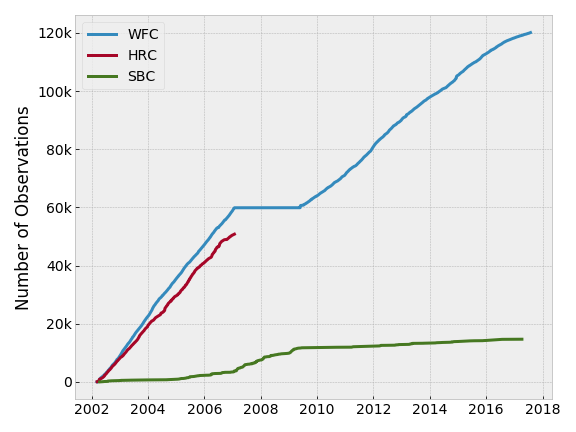
\includegraphics[width=3.5in]{./figures/num_obs.png}
\caption{The number of observations over time for each of the three detectors on ACS.}
\label{fig1}
\end{figure}

ACS data, along with all other data from the other HST instruments past and present
(e.g. The Wide Field Camera 3 (WFC3), The Cosmic Origins Spectrography (COS), etc.),
are primarily stored and publicly-available in the Barbara A. Mikulski Archive for
Space Telescopes (MAST)\footnote{named after the U.S. Senator from Maryland who has
been a pivitol political driving force behind the manned servicing missions, the
Hubble Space Telescope, and the forthcoming James Webb Space Telescope} (Barbara, 2017).
Through MAST, users can request and retreive data for any publicly-available dataset
via \texttt{ftp}, \texttt{sftp}, or DVD by mail\footnote{Not all HST data are publicly
available; most HST data of scientific targets are considered proprietary for up to
one calendar year, after which they are publicly released.}.  The ACS data, like most all other
astronomical data, are stored in the Flexible Image Transport System (FITS) filetype
(FITS, 2008).  This filetype has several unique characteristics, as will be
discuessed in section N.

The ACS Quicklook Project is a \texttt{python}-based application for discovering,
viewing, and querying all publicly-available ACS data.  It consists of several subsystems:
(1) A filesystem that stores ACS instrument data files and "Quicklook" JPEGs in an
organized Network File System (NFS), (2) A \texttt{MySQL} database that stores image
metadata of each observation, (3) A \texttt{python}/\texttt{Flask}-based web application
for interacting with the filesystem and database, and (4) A \texttt{python} code library
(named \texttt{acsql}) that contains code for connecting to the database, ingesting new
data, logging production code execution, and building/maintaining the database and web
application.  Each of these subsystems are explained in further detail in the Methodology
section of this paper.

This paper aims to outline and detail the ACS Quicklook project as part of the Towson
University Computer Science Masters Program Graduate Project.  The remaining subsections
in this chapter discuss the motivation and use cases for this application, as well as
details on the underlying data structure on top of which this project was built.  Chapter
2 discusses related work to this project and how the ACS Quicklook project differs from
existing similar applications.  Chapter 3 details the implementations of each of the
ACS Quicklook subsystems.  Chapter 4 outlines the results of the project, namely the
project deliverables.  Lastly, chapters 5 and 6 conclude the paper with a discussion
of possible extensions and modifications to the application.

It should be noted that the work that went into this project by the authors was
accomplished on behalf of the Space Telescope Science Institute (STScI) located in
Baltimore, Maryland.  STScI is the home institution for instrument, data, and user
support of HST, the forthcoming James Webb Space Telescope
(JWST), and MAST.  STScI is part of the Association of Universities for Research in
Astronomy (AURA).

\subsection{Motivation}

The motivation for the ACS Quicklook system is driven by several shortcomings of the
FITS file structure as well as the current capabilities of MAST from a specific
user perspective (inteded users and their use cases are discussed in section 1.2).
Some of these shortcomings are described below along with the intended way the
ACS Quicklook application will address them.

\textit{Data retreival letency:} Currently, users who wish to retreive data from
the MAST archive must submit a retreival request via the MAST online interface.
Once the retreival request is processed (usually automatically unless it is a
request of a large number of datasets), the data are either transfered to the user
directly via \texttt{sftp}, transfered to a "staging area" in which the user can
log into and copy the data via \texttt{ftp} at their leisure, or sent by mail via
DVD, depending on which option the user selects.  In the case of any one of these
options, the time between a download request and the the time in which the user
has fully retreived the data is a non-significant amount of time.  In the fastest
scenario of the \texttt{sftp} option, a typical request can take minutes to hours
to be completed.  The ACS Quicklook system attempts to circumnavigate this retreival
process by making the full data products instantly available via read-only access of
the filesystem subystem, as well as a subset of the data products (and corresponding
metadata) instantly available to view through the web application.

\textit{File I/O:} Users who

\textit{Data redundancy:} Something.

\textit{Data discovery:} Something


\subsection{Use Cases}
The intended user of ACS Quicklook are ACS instrument scientists, analysts,
or scientific users who wish to perform one or more of the following use cases:

1. View

\subsection{Data Structure}

\subsubsection{FITS file structure}

\subsubsection{FITS file headers}

% Figure for header example
\begin{figure}[!t]
\centering
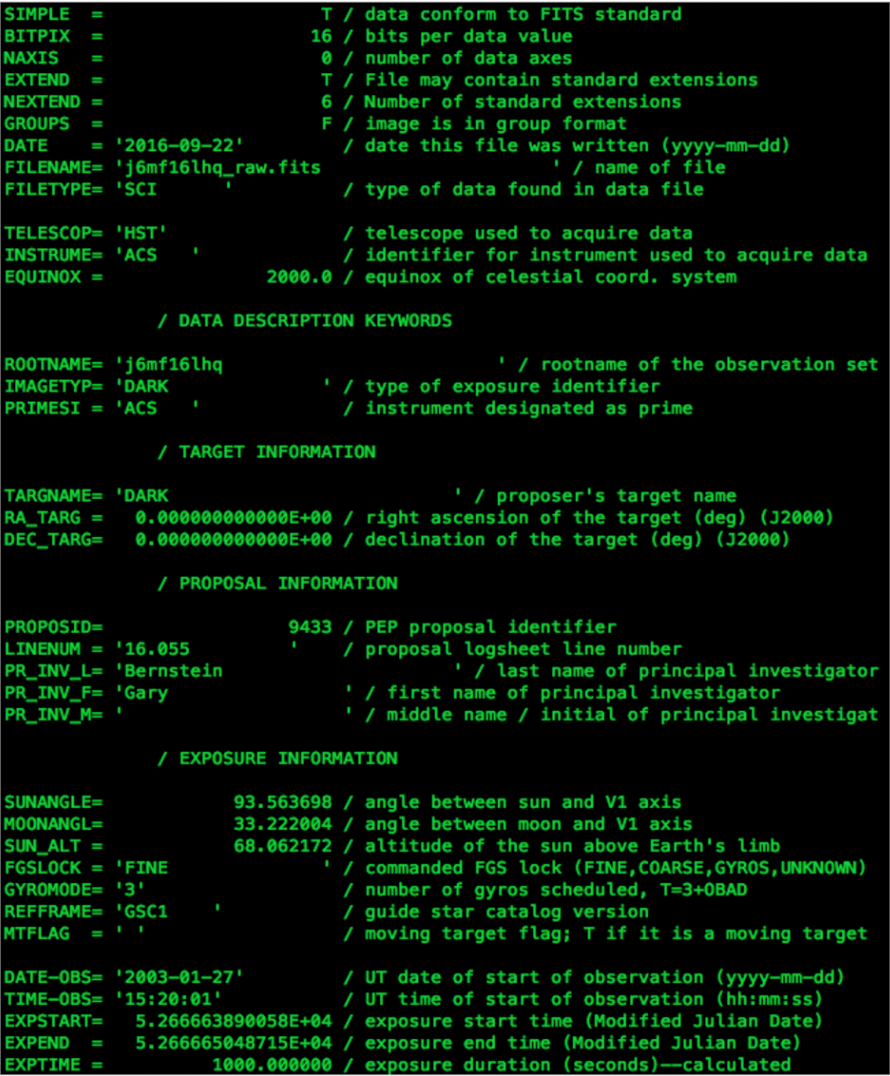
\includegraphics[width=3.5in]{./figures/header_example.png}
\caption{An example header.}
\label{fig1}
\end{figure}

\subsubsection{FITS filetypes for ACS}

\subsection{Key Metadata}



% Topics to discuss:

% 1. History of ACS
% 2. Motivation and users
% 3. Data Structure: FITS file and file extensions
% 4. Data Structure: FITS headers
% 5. Data Sturcture: FITS filetypes
% 6. Key Metadata
% 7. What this paper discusses


% Related Work
\section{Related Work}\label{sec:related_work}

Topics to discuss:

1. The MAST archive
2. The MAST portal
3. The WFC3/Quicklook project
4. Other Astronomy Institutions
5. How ACS/Quicklook is different

% Methodology
\section{Methodology}\label{sec:methodology}
Topics to discuss:

1. Version control
2. Programming and Documentation Standards
3. Filesystem: The MAST public Cache
4. Filesystem: Archive of JPEGs and Thumbnails
5. Database: Relational Schema
6. Database: MySQL + SQLAlchemy
7. Database: ORMs
8. Data ingestion software
9. Website:

% Figure for acsql database schema
\begin{figure}[!t]
\centering
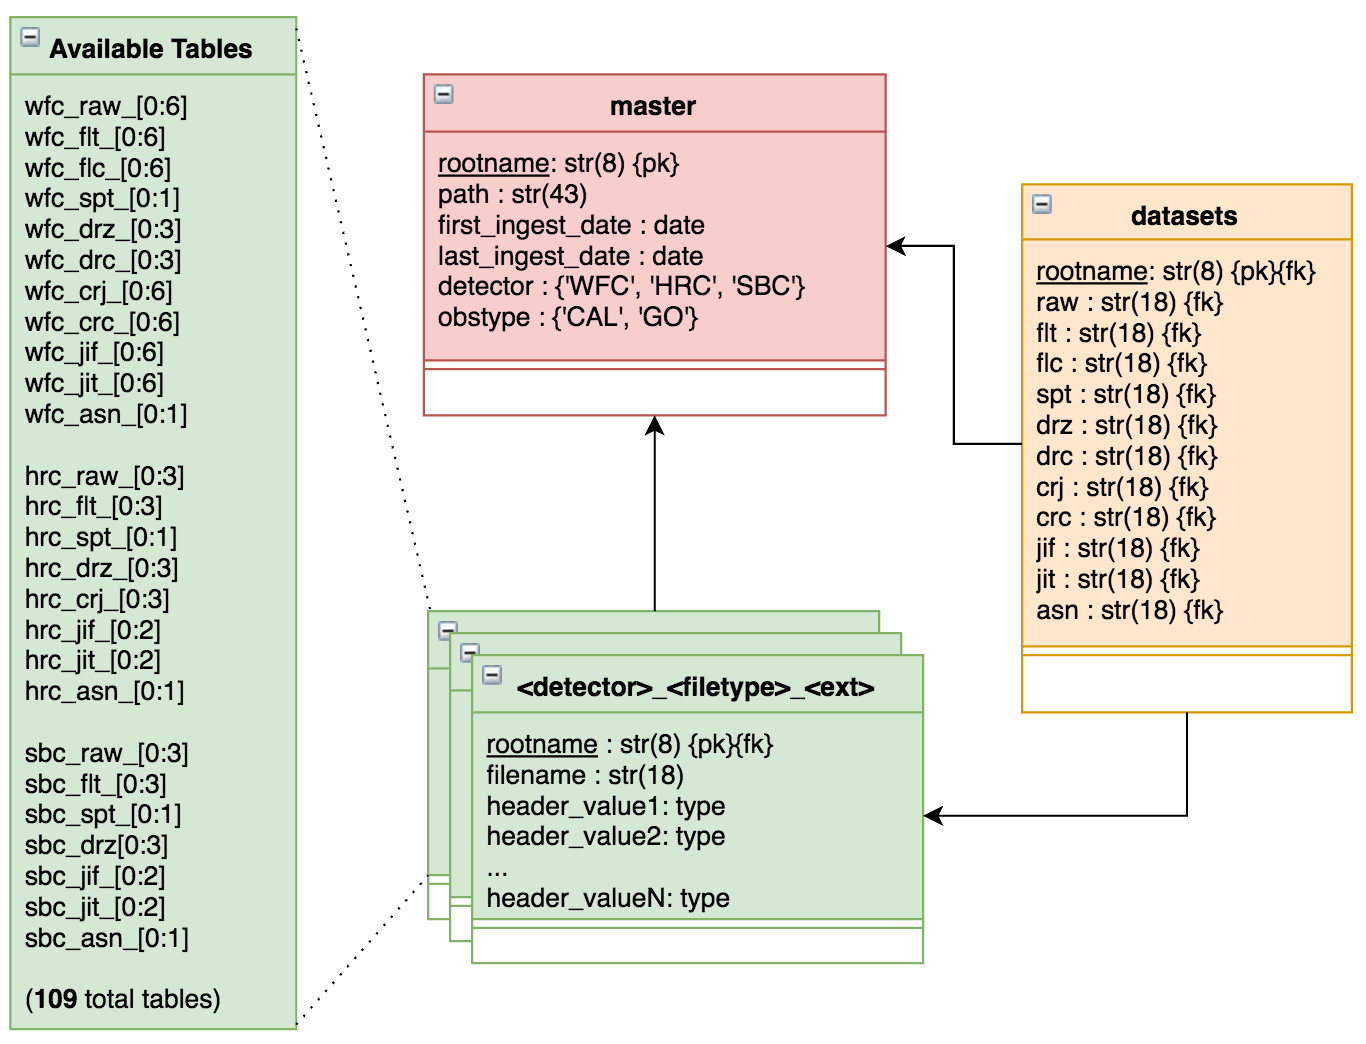
\includegraphics[width=3.5in]{./figures/schema.png}
\caption{The relational database schema for the \texttt{acsql} database.}
\label{fig1}
\end{figure}

% Results
\section{Results}\label{sec:results}

Topics to discuss:
1. GitHub repository
2. ReadTheDocs documentation repository
3. Quantification of Database records
4. Quantification of Code repository
5. Website location


%
%\begin{figure}[!t]
%\centering
%\includegraphics[width=2.5in]{myfigure}
% where an .eps filename suffix will be assumed under latex,
% and a .pdf suffix will be assumed for pdflatex; or what has been declared
% via \DeclareGraphicsExtensions.
%\caption{Simulation results for the network.}
%\label{fig_sim}
%\end{figure}


% An example of a double column floating figure using two subfigures.
% (The subfig.sty package must be loaded for this to work.)
% The subfigure \label commands are set within each subfloat command,
% and the \label for the overall figure must come after \caption.
% \hfil is used as a separator to get equal spacing.
% Watch out that the combined width of all the subfigures on a
% line do not exceed the text width or a line break will occur.
%
%\begin{figure*}[!t]
%\centering
%\subfloat[Case I]{\includegraphics[width=2.5in]{box}%
%\label{fig_first_case}}
%\hfil
%\subfloat[Case II]{\includegraphics[width=2.5in]{box}%
%\label{fig_second_case}}
%\caption{Simulation results for the network.}
%\label{fig_sim}
%\end{figure*}
%
%\begin{table}[!t]
%% increase table row spacing, adjust to taste
%\renewcommand{\arraystretch}{1.3}
% if using array.sty, it might be a good idea to tweak the value of
% \extrarowheight as needed to properly center the text within the cells
%\caption{An Example of a Table}
%\label{table_example}
%\centering
%% Some packages, such as MDW tools, offer better commands for making tables
%% than the plain LaTeX2e tabular which is used here.
%\begin{tabular}{|c||c|}
%\hline
%One & Two\\
%\hline
%Three & Four\\
%\hline
%\end{tabular}
%\end{table}


% Conclusion
\section{Conclusion}\label{sec:conclusion}
The conclusion goes here.

% Discussion
\section{Discussion}\label{sec:discussion}
Topics to discuss:

1. Possible simplification based on MAST archive
2. Possible extensions to other insturments

% Appendices
\appendices
\section{Proof of the First Zonklar Equation}
Appendix one text goes here.

% you can choose not to have a title for an appendix
% if you want by leaving the argument blank
\section{}
Appendix two text goes here.


% use section* for acknowledgment
\ifCLASSOPTIONcompsoc
  \section*{Acknowledgments}
\else
  \section*{Acknowledgment}
\fi
  The authors would like to thank...


% Can use something like this to put references on a page
% by themselves when using endfloat and the captionsoff option.
\ifCLASSOPTIONcaptionsoff
  \newpage
\fi


% Referecnes
\begin{thebibliography}{1}

\bibitem{IEEEhowto:avila}
Avila, R., et al., \emph{ACS Instrument Handbook}, Version 16.0 (Baltimore: STScI)

\bibitem{IEEEhowto:fits}
\emph{Definition of the Flexible Image Transport System (FITS): The FITS Standard}, 2008,
International Astronomical Union FITS Working Group, available at
\url{https://fits.gsfc.nasa.gov/standard30/fits_standard30aa.pdf}.

\bibitem{IEEEhowto:mast}
\emph{The Barbara A. Mikulski Archive for Space Telescopes}, [Online; accessed 2017-07-30],
available at \url{https://archive.stsci.edu/}.

\end{thebibliography}


% that's all folks
\end{document}
